\documentclass[11pt]{article}

\usepackage{fullpage}
\usepackage{rotating}   
\usepackage{amsmath}
\usepackage{amssymb}
\usepackage{amsthm}
\usepackage{fancyhdr}
\usepackage{algorithm}
\usepackage{algorithmic}
\usepackage{bm}
\usepackage{listings}
\usepackage{graphicx}
\usepackage{caption2}
\usepackage{subfigure}
\usepackage{float}
\usepackage{extpfeil}
\usepackage{color}
\usepackage[usenames,dvipsnames]{xcolor}


\newtheorem{theorem}{Theorem}[section]
\newtheorem{lemma}[theorem]{Lemma}
\newtheorem{corollary}[theorem]{Corollary}
\newtheorem{proposition}[theorem]{Proposition}
\newtheorem{definition}[theorem]{Definition}
\newtheorem{conjecture}[theorem]{Conjecture}
\newtheorem{remark}[subsection]{Remark}

%%
\newcommand\numberthis{\addtocounter{equation}{1}\tag{\theequation}}

%% define new symbols
\def\bx{\bm{x}}
\def\bb{\bm{b}}
\def\ba{\bm{a}}
\def\bc{\bm{c}}
\def\bf{\bm{f}}
\def\by{\bm{y}}
\def\bu{\bm{u}}
\def\bv{\bm{v}}
\def\BW{\bm{W}}
\def\BA{\bm{A}}
\def\bz{\bm{z}}
\def\BZ{\bm{Z}}
\def\BH{\bm{H}}
\def\BL{\bm{L}}
\def\BU{\bm{U}}
\def\BV{\bm{V}}
\def\BB{\bm{B}}
\def\BC{\bm{C}}
\def\BD{\bm{D}}
\def\BE{\bm{E}}
\def\BW{\bm{W}}
\def\BQ{\bm{Q}}
\def\BG{\bm{G}}
\def\BA{\bm{A}}
\def\BX{\bm{X}}
\def\BY{\bm{Y}}
\def\BQ{\bm{Q}}
\def\BI{\bm{I}}
\def\BR{\bm{R}}

%% define new brackets
\def\la{\left\langle}
\def\ra{\right\rangle}
\def\ln{\left\|}
\def\rn{\right\|}
\def\lb{\left(}
\def\rb{\right)}
\def\lsb{\left[}
\def\rsb{\right]}
\def\lcb{\left\{}
\def\rcb{\right\}}

%%
\DeclareMathOperator*{\argmin}{arg\,min}
\DeclareMathOperator*{\argmax}{arg\,max}

%%
\title{Homework V}
\author{Name: Shao Yanjun, Number: 19307110036}


\begin{document}
\maketitle

%------------------------------------
\begin{abstract}
This is Daniel's homework of  "Numerical Algorithms with Case Studies II".
\end{abstract}
%-------------------------------------
%=====================
\section{Problems}
\paragraph{Q1}
First, calculate the third-order derivative of $s(x)$.
\begin{align}
	s_0'''(x)&=12\frac{y_0}{h_0^3}-12\frac{y_1}{h_0^3}+6\frac{k_0}{h_0^2}+6\frac{k_1}{h_0^2}\\
	s_1'''(x)&=12\frac{y_1}{h_1^3}-12\frac{y_2}{h_1^3}+6\frac{k_1}{h_1^2}+6\frac{k_2}{h_1^2}\\
	s_{n-1}'''(x)&=12\frac{y_{n-1}}{h_{n-1}^3}-12\frac{y_{n}}{h_{n-1}^3}+6\frac{k_{n-1}}{h_{n-1}^2}+6\frac{k_{n}}{h_{n-1}^2}\\
	s_{n}'''(x)&=12\frac{y_{n}}{h_{n}^3}-12\frac{y_{n+1}}{h_{n}^3}+6\frac{k_{n}}{h_{n}^2}+6\frac{k_{n+1}}{h_{n}^2}
\end{align}
We apply the not-a-knot condition to $s_0'''(x)=s_1'''(x)$ and $s_(n-1)'''(x)=s_n'''(x)$, therefore,
\begin{align}
	2(\frac{y_0-y_1}{h_0^3}-\frac{y_1-y_2}{h_1^3})&=-k_0\frac{1}{h_0^2}+k_1(\frac{1}{h_1^2}-\frac{1}{h_0^2})+k_2\frac{1}{h_1^2}\\
	2(\frac{y_{n-1}-y_n}{h_{n-1}^3}-\frac{y_{n}-y_{n+1}}{h_n^3})&=-k_{n-1}\frac{1}{h_{n-1}^2}+k_n(\frac{1}{h_{n}^2}-\frac{1}{h_{n-1}^2})+k_{n+1}\frac{1}{h_{n}^2}
\end{align}
Maintain the rest of the equations, we have,
\begin{align}
\begin{pmatrix}
	-\frac{1}{h_0^2} & \frac{1}{h_1^2}-\frac{1}{h_0^2} & \frac{1}{h_1^2} & \cdots &0 &0 &0\\
	2\frac{1}{h_0} & 4\frac{1}{h_0}+4\frac{1}{h_1} & 2\frac{1}{h_1} & \cdots &0 &0 &0\\
	0 & 2\frac{1}{h_1} & 4\frac{1}{h_1}+4\frac{1}{h_2}& \cdots &0 &0 &0\\
	\vdots & \vdots &\vdots &\ddots &\vdots & \vdots &\vdots\\
		0 &0 &0 &\cdots & 4\frac{1}{h_{n-2}}+4\frac{1}{h_{n-1}} & 2\frac{1}{h_{n-1}} &0\\
	0 &0 &0 &\cdots & 2\frac{1}{h_{n-1}} & 4\frac{1}{h_{n-1}}+4\frac{1}{h_n} & 2\frac{1}{h_n}\\
	0 &0 &0 &\cdots & -\frac{1}{h_{n-1}^2} & \frac{1}{h_n^2}-\frac{1}{h_{n-1}^2} & \frac{1}{h_n^2} &
\end{pmatrix}
\begin{pmatrix}
	k_0\\k_1\\k_2\\\vdots\\k_{n-1}\\k{n}\\k_{n+1}
\end{pmatrix}
=\begin{pmatrix}
	2(\frac{y_0-y_1}{h_0^3}-\frac{y_1-y_2}{h_1^3})\\
	6(\frac{y_2-y_1}{h_1^2}+\frac{y_1-y_0}{h_0^2})
	\\\vdots\\
	6(\frac{y_{n+1}-y_n}{h_n^2}+\frac{y_n-y_{n-1}}{h_{n-1}^2})\\
	2(\frac{y_{n-1}-y_n}{h_{n-1}^3}-\frac{y_n-y_{n+1}}{h_n^3})
\end{pmatrix}
\end{align}
\paragraph{Q2}
The error is small for $f'(0)=0$, but the plot start to become strange and recognizable when $f'(0)$ was too far away.
\begin{figure}[H]
	\centering
	\subfigure[$f'(0)=1$]{
		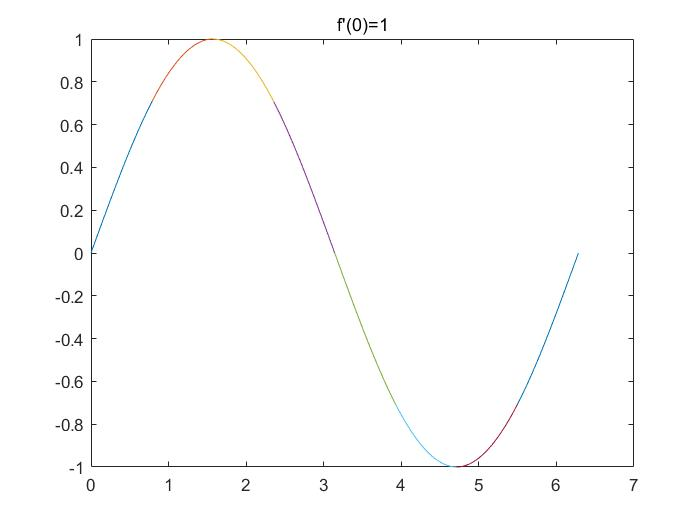
\includegraphics[width=0.35\linewidth]{f'(0)=1.jpg}
	}
	\subfigure[$f'(0)=0$]{
		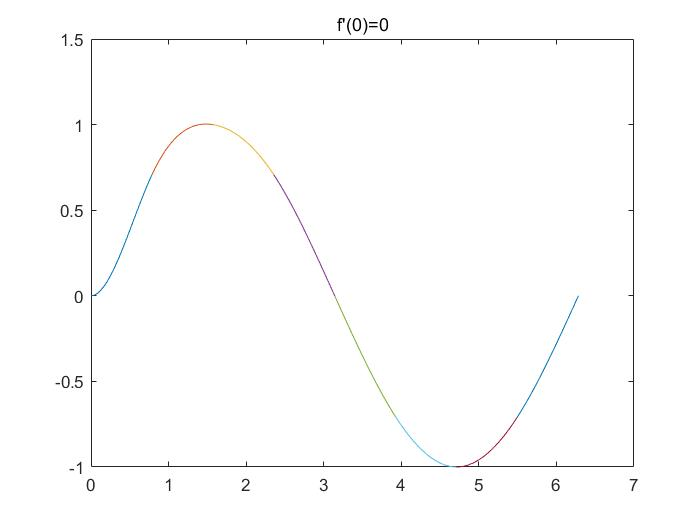
\includegraphics[width=0.35\linewidth]{f'(0)=0.jpg}
	}
	\subfigure[$f'(0)=-1$]{
		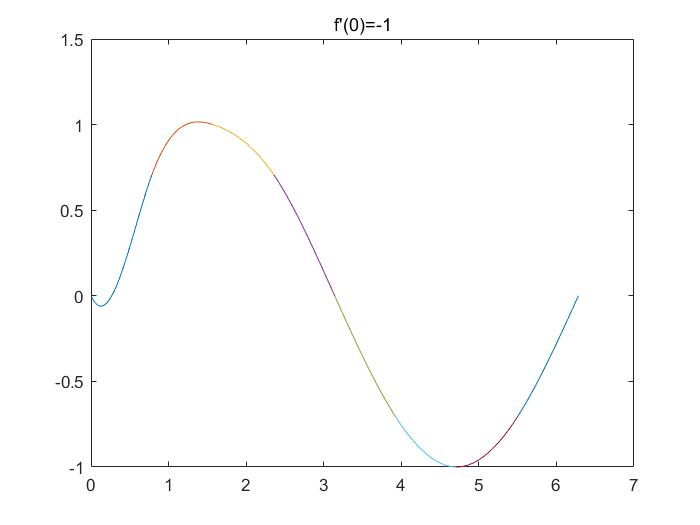
\includegraphics[width=0.35\linewidth]{f'(0)=-1.jpg}
	}
	\subfigure[$f'(0)=-5$]{
		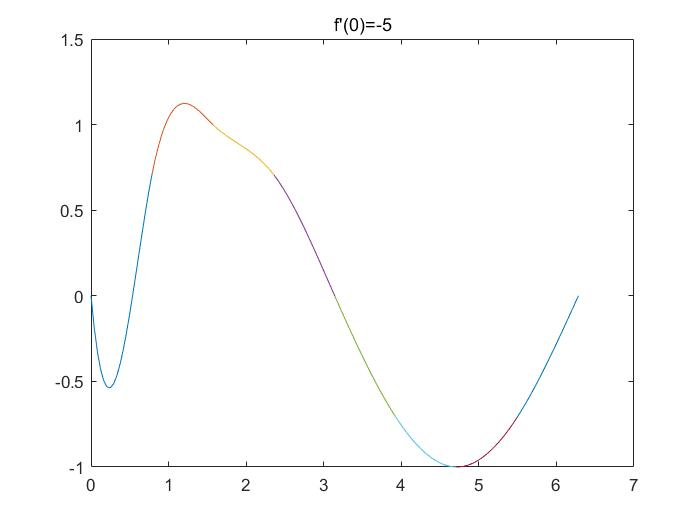
\includegraphics[width=0.35\linewidth]{f'(0)=-5.jpg}
	}
\end{figure}
\paragraph{Q3}
We assume that human body temperature remain parellel between two consecutive days. Also we connect $f(23)$ with $f(1+24)$ to maintain the periodicity. The dotted line represent estimated data, while the solid line represent the interpolated data.
\begin{figure}[H]
	\centering
	\subfigure[human body temperature in 2 days]{
		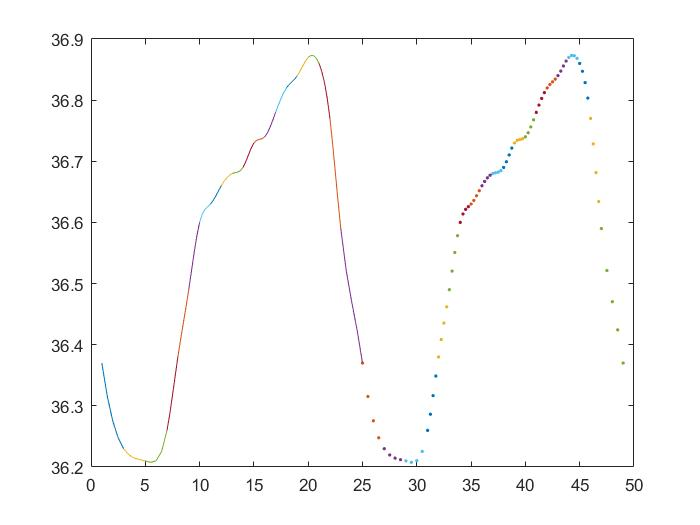
\includegraphics[width=0.5\linewidth]{body temperature.jpg}
	}
\end{figure}
\paragraph{Q4}
The result was rather funny if I set $p=100$ for $\|\cdot\|_p$, but the interpolation under $\|\cdot\|_2$ remain plausible.
\begin{figure}[H]
	\centering
	\subfigure[$\|\cdot\|_2$]{
		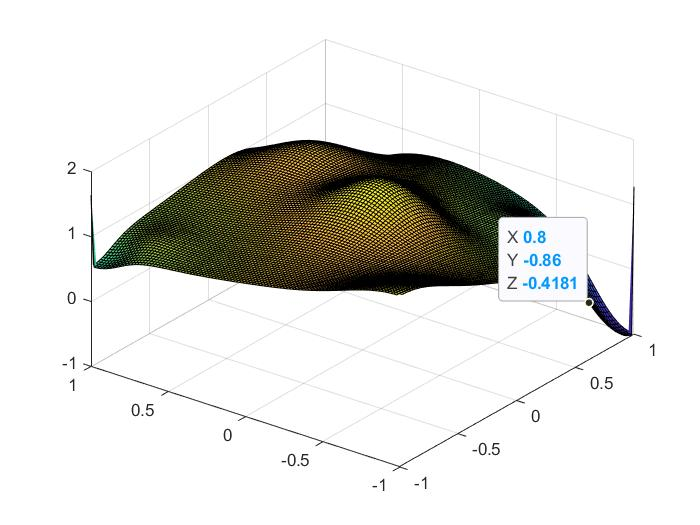
\includegraphics[width=0.4\linewidth]{norm2.jpg}
	}
	\subfigure[$\|\cdot\|_p$]{
	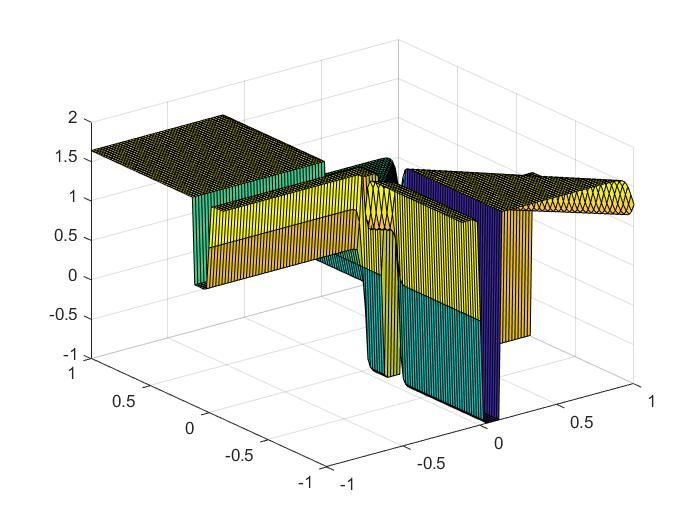
\includegraphics[width=0.4\linewidth]{square.jpg}
}
\end{figure}
\paragraph{Q5}
\subparagraph{(a)}
It turns out to be an "S" curve. Use the natural condition.
\begin{figure}[H]
	\centering
	\subfigure[curve 1]{
		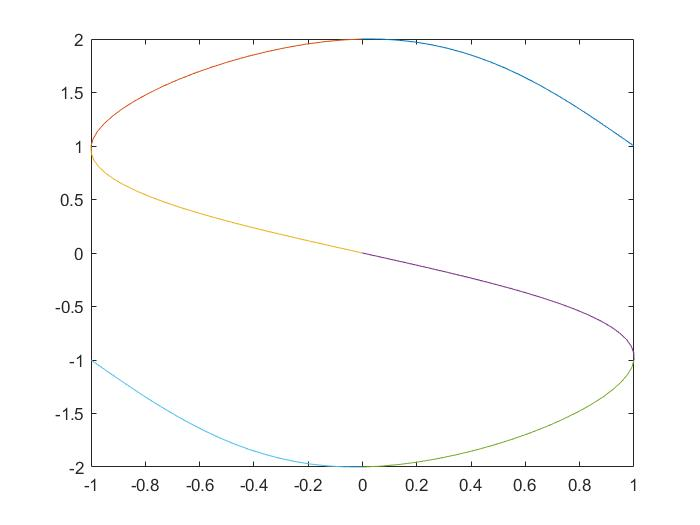
\includegraphics[width=0.6\linewidth]{plot1.jpg}
	}
\end{figure}
\subparagraph{(b)}
The bad news is that using natural condition makes the closed curve look not smooth enough. We applied periodic condition to make the head and tail meet smoothly.
\begin{figure}[H]
	\centering
	\subfigure[poor curve]{
		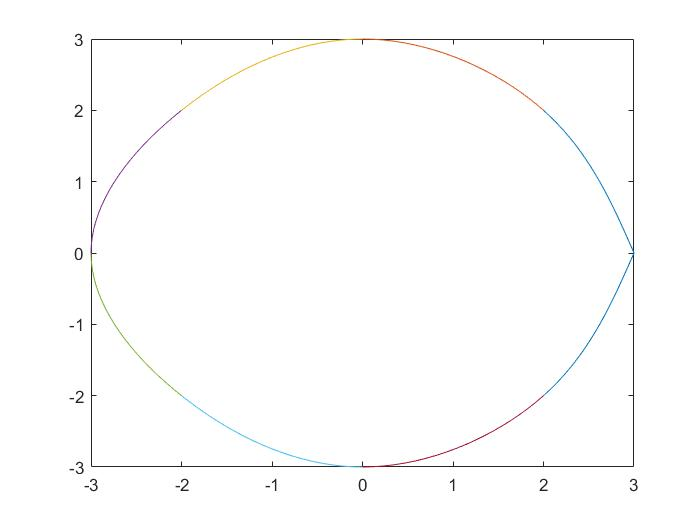
\includegraphics[width=0.4\linewidth]{plot2_notgood.jpg}
	}
	\subfigure[smooth curve]{
		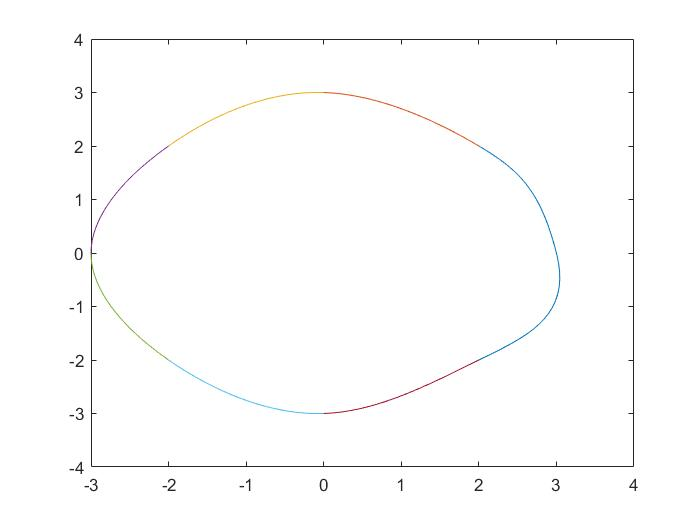
\includegraphics[width=0.4\linewidth]{plot2_potato.jpg}
	}
\end{figure}
%-------------------------------------
%=====================
\end{document}
